\begin{figure*}[th]
    \centering
    
    \begin{subfigure}[b]{\textwidth}
        \centering
        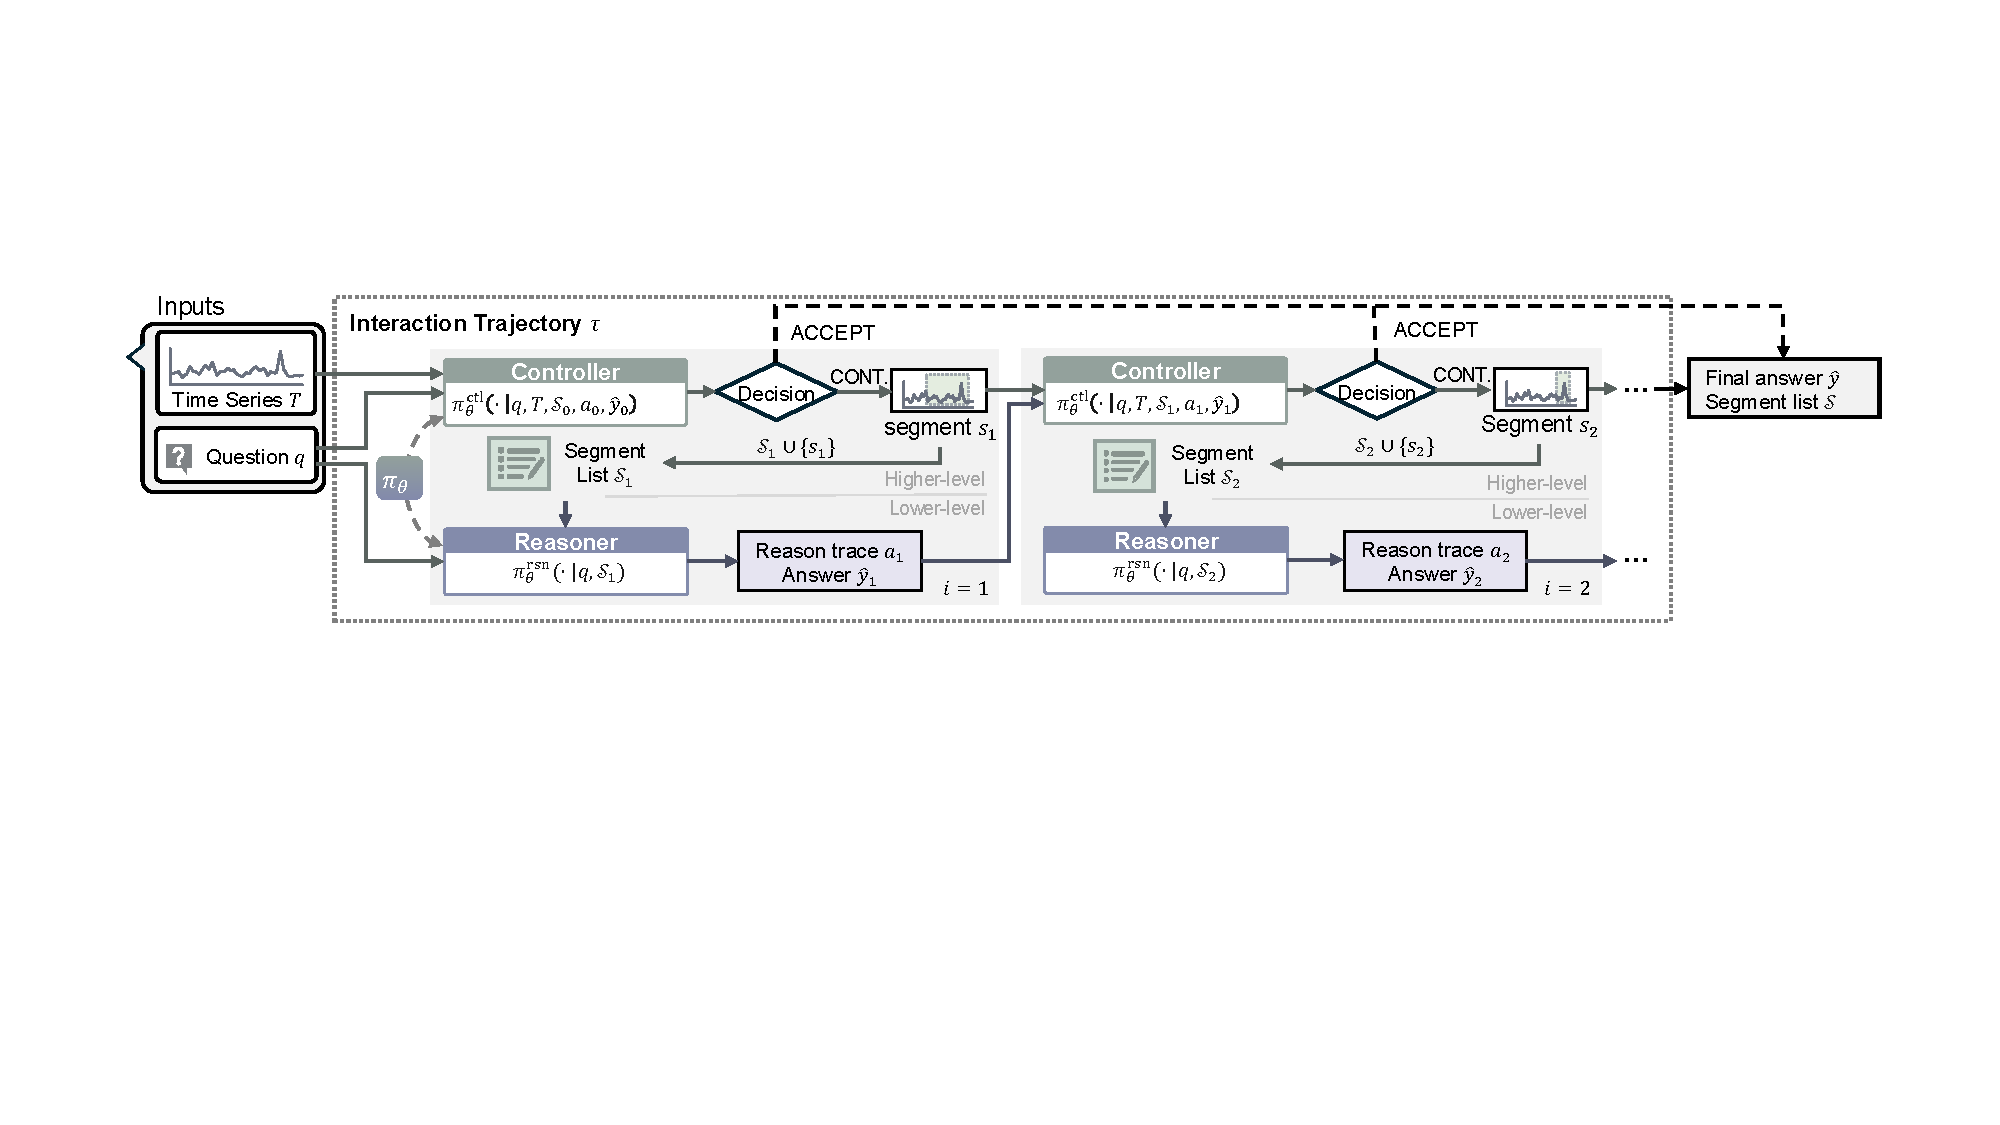
\includegraphics[width=\linewidth]{figs/fig2a_generation.pdf}
        \caption{Interaction Trajectory Rollout (Generation).}
        \label{fig:interact_traj}
    \end{subfigure}
    
    
    \begin{subfigure}[b]{\textwidth}
        \centering
        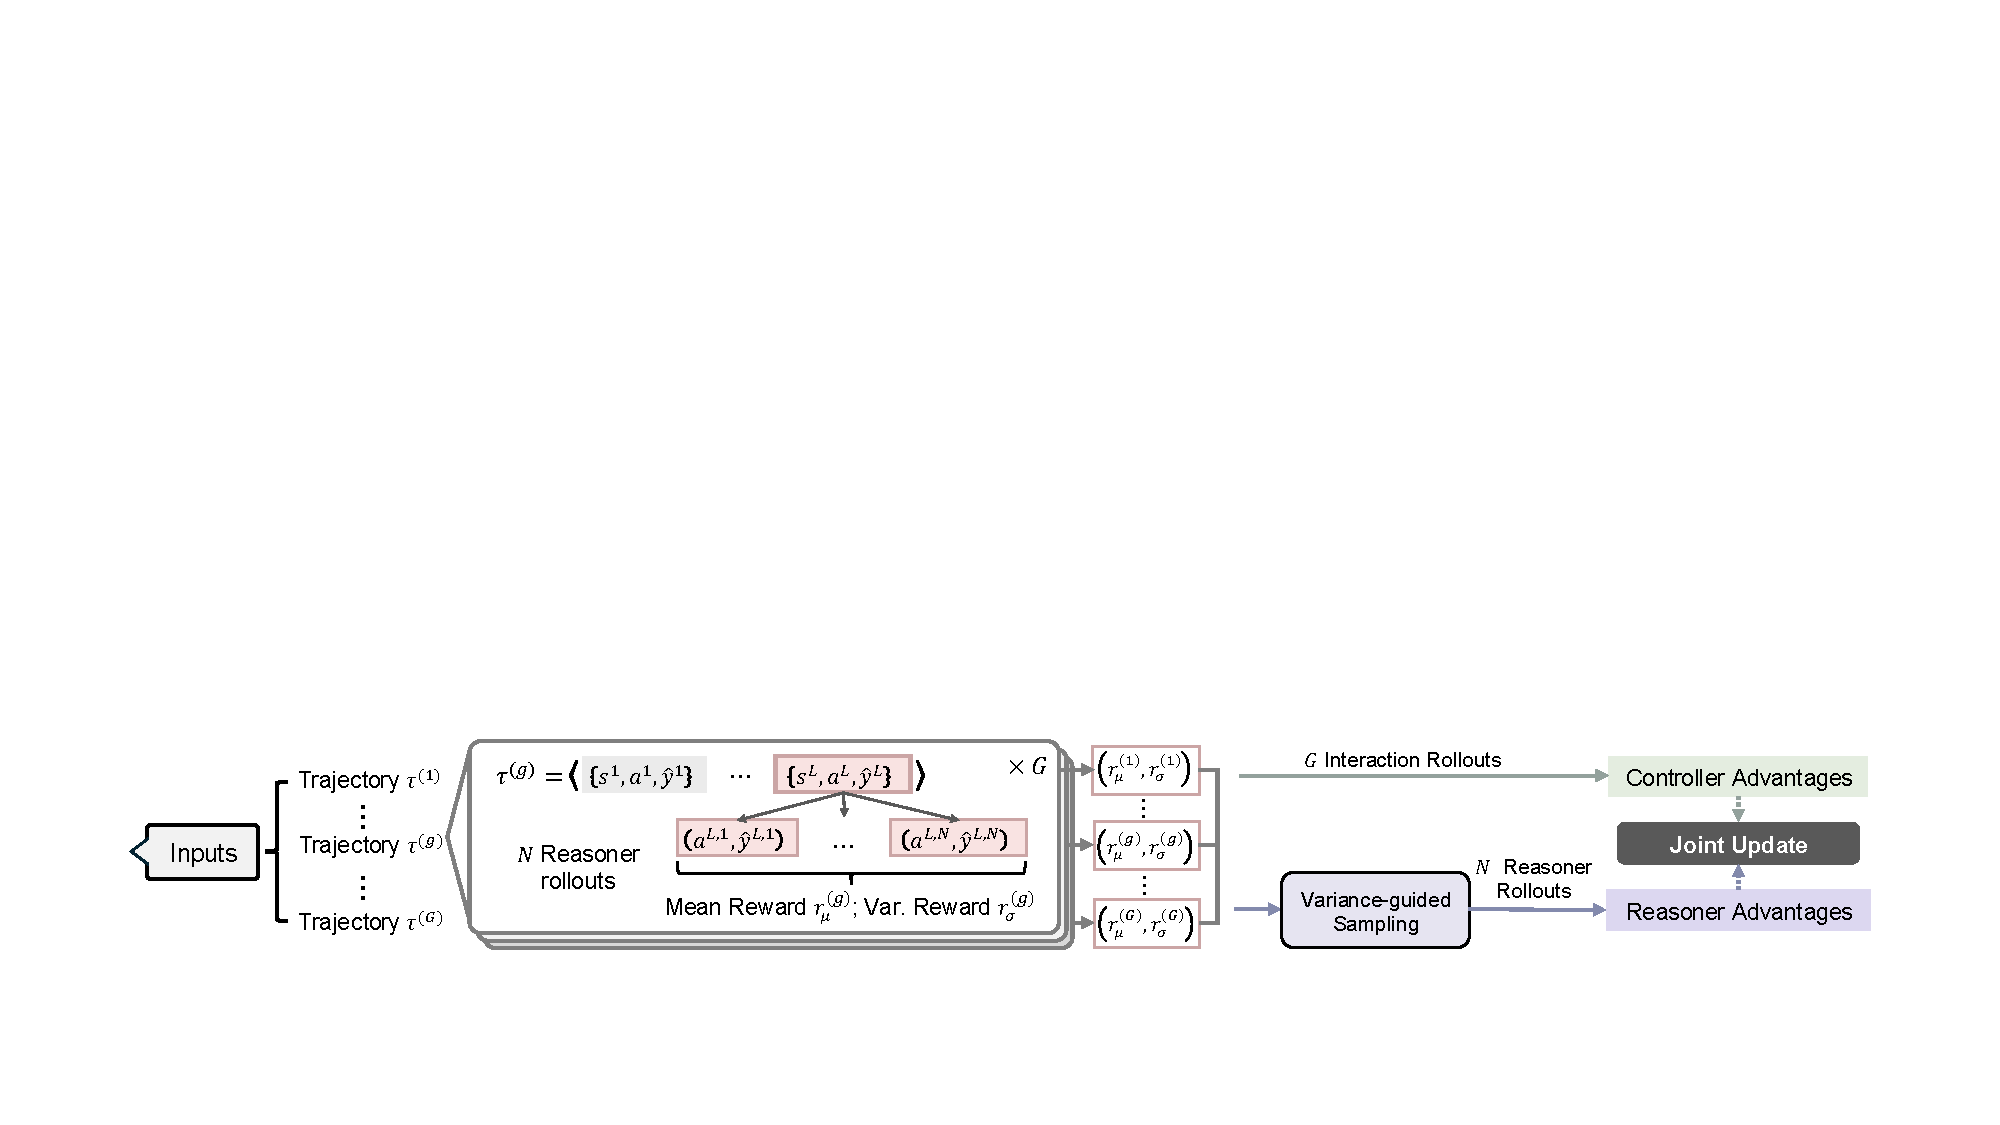
\includegraphics[width=\linewidth]{figs/fig2b_update.pdf}
        \caption{Unified Policy Update (Optimization).}
        \label{fig:policy_update}
    \end{subfigure}
    
    \caption{\textbf{Overview of \algoname.}
(a) Given a question and a time series, a high-level controller iteratively selects informative temporal segments, while a low-level reasoner produces intermediate reasoning traces and answers conditioned on the accumulated segment set. The controller decides whether to continue selecting or accept it as a final answer and segment list.
(b) For each training example, multiple reasoning rollouts are generated per controller trajectory. Reasoner rewards are group-normalized across reasoning rollouts, while controller rewards are computed using the associated reasoning outcomes and normalized across controller trajectories. Both signals are used for a joint policy update.}
\vspace{-5mm}
    \label{fig:method} 
\end{figure*}


\section{\algoname}
\label{sec:method}

\subsection{Problem Setup and Notation}
\label{sec:problem}

We study \emph{time-series reasoning} for a natural-language question $q$ paired with a time series
$T \in \mathbb{R}^{H \times V}$, where $H$ is the sequence length and $V$ is the number of variables.
A time-series large language model $\pi_\theta$ generates a textual response $Y$:
\begin{equation}
\pi_\theta(q, T) \to Y.
\end{equation}
In this paper, we focus on the univariate setting ($V=1$).

\xhdr{Time Series Reasoning}
We view reasoning as searching for a high-probability inference path that links $(q,T)$ to a correct answer.
Concretely, we introduce a latent sequence of intermediate steps $z=(z_1,\dots,z_L)$ and write:
\begin{equation}
p_\theta(Y \mid q,T)
\;=\;
\sum_{z \in \mathcal{Z}}
p_\theta(Y \mid z, q)\, p_\theta(z \mid q,T),
\label{eq:ts_reasoning_latent}
\end{equation}
where $z$ specifies \emph{how} the model inspects and interprets the signal before producing $Y$.


\xhdr{Segments}
A segment is a contiguous slice of the time series $T$, denoted
$s = T_{t_{\text{start}}:t_{\text{end}}}$ with $0 \le t_{\text{start}} < t_{\text{end}} \le H$.
We maintain an accumulated segment list $\mathcal{S}=[s^1,\dots,s^K]$ over multiple reasoning steps.



\subsection{Controller-Reasoner Roles in \algoname}
\label{sec:overview}

\algoname is a collaborative self-play model that equips a single policy model $\pi_\theta$ with both \emph{adaptive segment localization} and \emph{segment-conditioned reasoning}.
The same underlying model is invoked in two roles via role-specific prompting, yielding \emph{controller} $\pi_\theta^{\text{ctl}}$ and \emph{reasoner} $\pi_\theta^{\text{rsn}}$.
The controller decides which temporal segments to inspect and when to terminate the interaction, while the reasoner generates a reasoning trace and a final answer conditioned on the accumulated segments.

Each training iteration consists of (i) generating rollouts through Controller-Reasoner interaction and (ii) computing a joint policy update. Figure~\ref{fig:method} illustrates the rollout and update structure, and Algorithm~\ref{alg:ouralgopsuedocode} summarizes the optimization process.

\subsection{Interaction Trajectory Rollout}
\label{sec:interactionrollout}


For a given question-time series pair $(q, T)$, an \emph{interaction trajectory} $\tau$ is a sequence of Controller-Reasoner interaction rounds indexed by $i=1,2,\dots,L$, where $L$ is the realized number of rounds until termination.

\xhdr{Controller Step}
At round $i$, the Controller receives the current state:
\begin{equation}
x_{i}^{\text{ctl}}=\bigl(q,T,\mathcal{S}_{i-1},a_{i-1},\hat{y}_{i-1}\bigr),
\label{eq:ctl_state}
\end{equation}
where $(\mathcal{S}_{0}, a_{0},\hat{y}_{0})$ are empty at initialization. In all subsequent interaction rounds $i > 1$, $a_{i-1}$ and $\hat{y}_{i-1}$ are the reasoning trace and answer provided by the Reasoner in the previous round $i-1$.
The controller then outputs a reasoning trace $u_i$ and a termination decision
$d_i\in\{\textsc{Continue},\textsc{Accept}\}$.
If $d_i=\textsc{Continue}$, it additionally proposes a new segment $s_i$:
\begin{equation}
(u_i,d_i,s_i)\sim \pi^{\text{ctl}}_\theta(\cdot\mid x_{i}^{\text{ctl}}),
\label{eq:ctl_out}
\end{equation}
and we append the new segment to the segment list $\mathcal{S}_{(i)} \leftarrow \mathcal{S}_{i-1} \cup \{s_i\}$.
If $d_i=\textsc{Accept}$, the interaction terminates and the answer outputted by the Reasoner step in the previous round, $\hat{y}_{i-1}$, is accepted as the final answer.

\xhdr{Reasoner Step}
If $d_i=\textsc{Continue}$, the Reasoner is invoked with the updated segment list $\mathcal{S}_{i}$ and produces a reasoning trace $a_i$ and answer $\hat{y}_i$:
\begin{equation}
(a_i,\hat{y}_i)\sim \pi^{\text{rsn}}_\theta(\cdot\mid q,\mathcal{S}_{i}).
\label{eq:rsn_continue}
\end{equation}

Formally, we define an interaction trajectory as:
\begin{equation}
\tau = \bigl\{(u_i, s_i, d_i, a_i, \hat{y}_i)\bigr\}_{i=1}^{L},
\qquad d_L=\textsc{Accept}.
\end{equation}
We further define two sub-trajectories of an interaction trajectory: \emph{controller trajectory} as $\tau_{\text{ctl}} = \{(u_i, s_i, d_i)\}_{i=1}^{L}$, and the \emph{reasoner trajectory @ round $i$} as $\tau_{\text{rsn, i}} = (a_i, \hat{y}_i)$.


\subsection{Reward Functions}
\label{sec:rewardfunctions}

We define rewards for the two roles based on answer correctness, reliability across repeated trials, and format compliance.

\xhdr{Correctness Reward}
Given a question $q$, gold answer $y^*$, and prediction $\hat{y}$, we define the correctness reward as:
\begin{equation}
C(q,y^*,\hat{y}) = \mathbf{1}\!\left[\hat y = y^*\right].
\label{eq:correctness}
\end{equation}
%
\xhdr{Reliability Reward}
Given $q$ and a segment list $\mathcal{S}$, we define reliability as the expected correctness of the Reasoner under repeated sampling conditioned on $(q,\mathcal{S})$.
In practice, we estimate it with $N$ independent rollouts $\hat{y}^{(n)} \sim \pi_\theta^{\text{rsn}}(\cdot \mid q,\mathcal{S}), n=1,\dots,N$ and then calculate:
\begin{equation}
\begin{split}
D(q,\mathcal{S},y^*)
=
\frac{1}{N}\sum_{n=1}^{N}\mathbf{1}\!\left[\hat y^{(n)} = y^*\right]
\\
=
\frac{1}{N}\sum_{n=1}^{N}C(q,y^*,\hat{y}^{(n)}).
\end{split}
\label{eq:reliability}
\end{equation}
A higher reliability reward indicates that the selected segments $\mathcal{S}$ make the Reasoner consistently produce the correct answer under sampling noise, and we use it as the learning signal for the Controller.


\xhdr{Controller Format Score}
Each controller step receives a per-step format score $f_i$ that captures minor but executable errors such as multiple reasoning blocks (see Appendix~\ref{app:format_score}). 
Given controller trajectory $\tau_{\text{ctl}}=\{(u^i,d^i,s^i)\}$, we additionally define a critical violation indicator $\mathbb{I}_{\text{viol}}(\tau_{\text{ctl}})\in\{0,1\}$ that flags non-executable outputs (full list in Appendix~\ref{app:format_score}). We then define:

\begin{equation}
F_{\text{ctl}}(\tau_{\text{ctl}})
=
\bigl(1-\mathbb{I}_{\text{viol}}(\tau_{\text{ctl}})\bigr)\cdot
\frac{1}{L}\sum_{i=1}^{L} f_i
\;-\;
\mathbb{I}_{\text{viol}}(\tau_{\text{ctl}}).
\label{eq:ctrl-format-ind}
\end{equation}
%
\xhdr{Controller Reward}
The controller reward is defined as:
\begin{equation}
R_{\text{ctl}}(\tau_{\text{ctl}}, D) =
\begin{cases}
-1 & \text{if } F_{\text{ctl}}(\tau_{\text{ctl}}) < 0,\\[4pt]
w_D\,D + w_f\,F_{\text{ctl}}(\tau_{\text{ctl}}) & \text{otherwise},
\end{cases}
\label{eq:ctrl-reward}
\end{equation}
where $w_D, w_f$ are tunable hyperparameters.
%

\xhdr{Reasoner Reward}
Given a final-round reasoner trajectory $\tau_{\text{rsn}}=(a,\hat{y})$ with correctness $c=C(q,y^*,\hat{y})$,
\begin{equation}
R_{\text{rsn}}(\tau_{\text{rsn}}, c) = w_c\,c + w_e\,F_{\text{rsn}}(\tau_{\text{rsn}}),
\label{eq:rsn-reward}
\end{equation}
where $F_{\text{rsn}}$ scores format compliance (Appendix~\ref{app:format_score}) and $w_c, w_e$ are tunable hyperparameters.


\subsection{Hierarchical Policy Optimization}
\label{sec:policyoptimization}

As shown in Fig.~\ref{fig:policy_update}, we use nested rollouts to obtain separate learning signals for the Controller and Reasoner behavior, and combine them into a joint update. Decomposing the parameter update in this way enables more precise credit assignment, as advantage signals are propagated only to the relevant tokens for each role.

\xhdr{Nested Rollouts}
For each training example $(q,T,y^*)$, we first sample $G$ interaction trajectories
$\{\tau^{(g)}\}_{g=1}^{G}$ following Sec.~\ref{sec:interactionrollout}.
Let the terminating round of $\tau^{(g)}$ be $L^{(g)}$, and let the final segment list be $\mathcal{S}^{(g)}_{L^{(g)}}$
($\textsc{Accept}$ does not add a new segment).
For each interaction trajectory $g$, we then resample the Reasoner $N$ times conditioned on the same final segment list, and denote these final-round reasoner trajectories as
$\tau_{\text{rsn},L^{(g)}}^{(g,n)}=(a_{L^{(g)}}^{(g,n)},\hat{y}_{L^{(g)}}^{(g,n)}), n=1,\dots,N$.

We then compute the mean and variance correctness rewards for reasoner trajectories, i.e., $r_\mu^{(g)}$ and $r_\sigma^{(g)}$, where $r_\mu^{(g)}$ equals the reliability reward in Eq.~\eqref{eq:reliability} for the final segments $\mathcal{S}^{(g)}_{L^{(g)}}$ produced in rollout $g$.


\xhdr{Higher-Level Advantage Calculation for Controller}
The Controller is optimized as a high-level policy that iteratively localizes segments across multiple interactions with the Reasoner and decides when the current information is sufficient.
For each interaction rollout $g\in\{1,\dots,G\}$, we compute a Controller reward
$r_{\text{ctl}}^{(g)}= R_{\text{ctl}}\!\bigl(\tau_{\text{ctl}}^{(g)},\, r_\mu^{(g)}\bigr)$ for controller trajectory $\tau_{\text{ctl}}^{(g)}$.
We then form group-relative advantages
$\{\hat{A}_{\text{ctl}}^{(g)}\}_{g=1}^G$ according to Appendix~\ref{app:controller_advantages}.

\xhdr{Lower-Level Advantage Calculation for Reasoner}
The Reasoner is optimized as a low-level policy that maximizes answer quality and formatting conditioned on the segments selected by the Controller.
Unlike the Controller, the Reasoner update optimizes only the final-round rollouts under a fixed segment list, disentangling the optimization of Reasoner behavior from the variance in quality of the segments selected by the Controller.
For each interaction rollout $g$, we draw $N$ independent final-round Reasoner rollouts
$\{\tau_{\text{rsn},L^{(g)}}^{(g,n)}\}_{n=1}^{N}$ under the same $\mathcal{S}$.

Using all $G\times N$ rollouts for every update can be memory-intensive, and many groups provide limited learning signal when their rewards are nearly identical. We therefore update the Reasoner using a single group $g^*$ selected by \emph{variance-guided sampling}, which prioritizes interaction trajectory that induce diverse outcomes and thus yield a more informative within-group advantage signal:
%
\begin{equation}
p(g) \;\propto\; r_\sigma^{(g)},
\end{equation}
where $r_\sigma^{(g)}$ is the variance of correctness across the $N$ rollouts in group $g$. For the sampled group $g^*$, we compute a Reasoner reward for each trajectory
$\tau_{\text{rsn}}^{(g^*,n)}$:
\begin{equation}
r_{\text{rsn}}^{(g*,n)} \;=\; R_{\text{rsn}}\!\Bigl(\tau_{\text{rsn},L^{(g)}}^{(g^*,n)},\, C\bigl(q,y^*,\hat{y}_{L^{(g)}}^{(g^*,n)}\bigr)\Bigr),
\end{equation}
and form group-relative advantages $\{\hat{A}_{\text{rsn}}^{(g^*,n)}\}_{n=1}^N$ according to Appendix~\ref{app:reasoner_advantages}.

\xhdr{Joint Update}
Finally, we aggregate the Controller advantages $\{\hat{A}_{\text{ctl}}^{(g)}\}_{g=1}^G$ and the Reasoner advantages $\{\hat{A}_{\text{rsn}}^{(g^*,n)}\}$ into a joint update of the shared parameters $\theta$ of $\pi_\theta$ that maximizes the objectives in Appendix~\ref{app:objectives}. Crucially, our Controller advantage signals are propagated across the Controller outputs from \emph{all} rounds $i \in \{1, ..., L^{(g)}\}$ in each interaction trajectory $\tau^{(g)}$, optimizing the role's behavior for incrementally choosing segments over multiple interactions that eventually result in the best segment \emph{set} long-term. In contrast, the Reasoner advantage signals are propagated only to the Reasoner outputs from the last round $L^{(g)}$ in each $\tau^{(g)}$, optimizing the role's behavior myopically to encourage focused, granular reasoning during question-answering. This hierarchical optimization setup is advantageous compared to previous self-play approaches for reasoning-based post-training that optimize both roles myopically, which would not be compatible for iterative segment selection.

\begin{algorithm}
    \caption{Hierarchical Policy Optimization}
    \label{alg:ouralgopsuedocode}
    \small
    \begin{algorithmic}
        \REQUIRE initial policy model $\pi_{\theta_\text{init}}$, question $q$
        \STATE $\pi_{\theta} \gets \pi_{\theta_\text{init}}$
        \FOR{$g = 1, 2, ..., G$}
            \STATE $\tau^{(g)} \gets$ interaction rollout of length $L^{(g)}$ using $\pi_{\theta}$
            \FOR{$n = 1, 2, ..., N$}
                \STATE $\tau_{rsn, L^{(g)}}^{(g, n)} \gets (a_{L^{(g)}}^{(g,n)},\hat{y}_{L^{(g)}}^{(g,n)}) $ (resampled reasoner rollout @ iter. $L^{(g)}$)
                \STATE $ r_{\text{rsn}}^{(g,n)} \gets R_{\text{rsn}}\!\Bigl(\tau_{\text{rsn}}^{(g,n)},\, C\bigl(q,y,\hat{y}^{(g,n)}\bigr)\Bigr)$
            \ENDFOR
            \STATE $r_\mu^{(g)} \gets \text{Mean}(\{C\bigl(q,y,\hat{y}_{L^{(g)}}^{(g,n)}\bigr)\Bigr)\}_{n=1}^N)$
            \STATE $r_\sigma^{(g)} \gets \text{Var}(\{C\bigl(q,y,\hat{y}_{L^{(g)}}^{(g,n)}\bigr)\Bigr)\}_{n=1}^N)$
            \STATE $r_\text{ctl}^{(g)} \gets R_{\text{ctl}}\!\bigl(\tau_{\text{ctl}}^{(g)},\, r_\mu^{(g)}\bigr)$
        \ENDFOR
        \STATE Calculate advantages $\hat{A}_{\text{ctl}}^{(g)}$ using $\{r_\mu^{(g)}\}_{g=1}^G$
        \STATE Sample $g^* \sim \{1, 2, ..., G\}: p(g) \propto r_\sigma^{(g)}$
        \STATE Calculate advantages $\hat{A}_{\text{rsn}}^{(g^*,n)}$ using $\{r_{\text{rsn}}^{(g^*,n)}\}_{n=1}^N$
        \STATE Joint update using $\hat{A}_{\text{ctl}}^{(g)}$ and $\hat{A}_{\text{rsn}}^{(g^*,n)}$
    \end{algorithmic}
\end{algorithm}

